% Standalone manuscript: figures, listings, and bibliography are embedded.
% Compile with pdfLaTeX; no shell escape, BibTeX, or external assets required.
\documentclass[11pt,letterpaper]{article}
\usepackage[T1]{fontenc}
\usepackage{lmodern}
\usepackage[margin=1in]{geometry}
\usepackage{microtype}
\usepackage{amsmath,amssymb,amsthm}
\usepackage{booktabs,array}
\usepackage{xcolor}
\usepackage{graphicx}
\usepackage{tikz}
\usetikzlibrary{arrows.meta,positioning}
\usepackage{pgfplots}
\pgfplotsset{compat=1.18}
\usepackage{listings}
\usepackage{enumitem}
\usepackage{fancyhdr}
\usepackage{url}
\usepackage[colorlinks=true,linkcolor=blue!45!black,citecolor=blue!45!black,urlcolor=blue!45!black]{hyperref}
\definecolor{ink}{HTML}{214E70}
\definecolor{accent}{HTML}{B85C38}
\definecolor{pale}{HTML}{F3F5F7}
\hypersetup{pdftitle={Fourier: Resumable FFT Scheduling for Real-Time Spectral Analysis},pdfauthor={Christian Kauten},pdfsubject={Technical report on cooperative FFT scheduling, latency, and reproducible evaluation},pdfkeywords={FFT, STFT, cooperative scheduling, real-time audio, spectrum analysis, VCV Rack}}
\pagestyle{fancy}
\fancyhf{}
\fancyhead[L]{\small\textsc{Fourier: Resumable FFT Scheduling}}
\fancyhead[R]{\small Technical report}
\fancyfoot[C]{\thepage}
\setlength{\headheight}{14pt}
\setlength{\emergencystretch}{2em}
\setlist{nosep}
\newtheorem{proposition}{Proposition}
\newcommand{\code}[1]{\texttt{#1}}
\newcommand{\ceil}[1]{\left\lceil #1\right\rceil}
\newcommand{\floor}[1]{\left\lfloor #1\right\rfloor}
\newcommand{\repo}{\url{https://github.com/Kautenja/ArhythmeticUnits-Fourier}}
\lstset{basicstyle=\ttfamily\footnotesize,keywordstyle=\color{ink}\bfseries,commentstyle=\color{black!55},stringstyle=\color{accent},backgroundcolor=\color{pale},frame=single,rulecolor=\color{black!15},breaklines=true,columns=fullflexible,keepspaces=true,showstringspaces=false,tabsize=4,captionpos=b,xleftmargin=0.5em,xrightmargin=0.5em}
\title{\textbf{Fourier: Resumable FFT Scheduling\\for Real-Time Spectral Analysis}}
\author{Christian Kauten\\\small Arhythmetic Units\\\small\href{mailto:arhythmetic.units@gmail.com}{arhythmetic.units@gmail.com}}
\date{September 28, 2026\\\small Technical report, manuscript version 1}

\begin{document}
\maketitle
\begin{abstract}
A Fourier transform that is inexpensive in aggregate can still impose an
undesirable burst of work on a real-time audio engine. This report examines a
resumable radix-2 implementation in Fourier, an open-source spectrum analyzer
and spectrogram plugin for VCV Rack. The implementation retains its butterfly
traversal state between engine calls and assigns a fixed number of butterflies
to each call. We describe the complex and real transforms, prove the
operation-count completion bound, and distinguish the requested computation
horizon from the actual spacing of analysis frames. A finite-window latency
model exposes the cost of deferring a completed frame's transform. Source
analysis identifies preparation, reconstruction, smoothing, and display
conversion as residual bursts outside the butterfly budget. Reproducible scalar
experiments verify spectral agreement and illustrate the difference between
aggregate work and observed peak call duration. Across four transform lengths
on one Apple M1 Pro system, incremental execution substantially reduces the
median of observed per-run peak call durations relative to the same transform
run to completion, while retaining linear-time boundary work. These results
support a narrow engineering conclusion: resumability offers useful control of
work placement, but a butterfly budget alone is neither an exact frame clock
nor a hard real-time guarantee. The contribution is an implementation study and
reproducible scheduling analysis, situated within established work on
time-distributed FFTs, rather than a new Fourier factorization.
\end{abstract}
\noindent\textbf{Keywords:} fast Fourier transform; short-time Fourier transform;
cooperative scheduling; real-time audio; spectral analysis; VCV Rack.

\section{Introduction}
A real-time audio system must complete the work associated with an audio buffer
before the next buffer is required. A spectral analyzer participates in this
constraint even when it produces no audio output: computation performed on the
engine thread competes with oscillators, filters, and other processors. The
relevant resource is therefore not only transforms per second, but also how
transform work is distributed across the host's processing intervals.

A conventional batch FFT interface accepts a complete frame and returns a
complete spectrum. Such an interface is appropriate when the call fits the
available budget, or when a worker thread can perform the analysis with an
acceptable publication delay. A sample-based plugin may instead benefit from
retaining an unfinished transform and performing a small amount of it whenever
the host processes another sample. This makes scheduling visible at the DSP
interface without introducing an additional thread.

Fourier implements this latter design. Its Fourier module computes four
independent spectra using SIMD lanes; its Spectre module maintains a scalar
spectrogram history. Both use the same templated real FFT. The implementation
is compact enough that its scheduling behavior can be derived directly from
its state machine, including behaviors not captured by its nominal ``hop
length'' parameter.

This report makes three contributions. First, it gives a precise account of
the transform state, work count, frame cadence, and latency of the implemented
scheduler. Second, it separates the bounded butterfly kernel from the larger
analysis pipeline, identifying where the latter retains concentrated work.
Third, it supplies deterministic numerical checks and paired timing
measurements, with the source and raw observations needed to reproduce them.
These are software-engineering contributions; we make no claim to a new FFT
factorization, the invention of time distribution, or a general performance
advantage over optimized transform libraries.

The evaluated DSP source is identified by revision
\code{b52e49c548ae}. The accompanying artifact records
SHA-256 digests of the experiment and math headers. The report concerns that
source snapshot, not every historical release bearing the same plugin version.

\section{Related Work and Positioning}
\label{sec:related}
Cooley and Tukey's factorization is the mathematical foundation of the complex
transform used here~\cite{cooley1965}. Real-input symmetry and real FFT
algorithms have a substantial independent literature, including Sorensen
et al.~\cite{sorensen1987}. Short-time Fourier analysis and synthesis provide
the frame-based interpretation~\cite{allen1977}; window selection and its
spectral consequences are treated systematically by Harris~\cite{harris1978}.
The packing and windowing used in Fourier are applications of this established
body of work.

Time-distributed FFT computation also predates this implementation. Lo and Lee
construct split-radix butterfly work as data become available during
acquisition~\cite{lo1998,lo1999}. Their moving FFT additionally combines
real-time scheduling with recursive reuse across shifted
frames~\cite{lomoving1999}. These methods are closer to acquisition-aware
computation than the present implementation, which first snapshots a full
window and then defers its arithmetic.

Hurchalla describes a time-distributed FFT for low-latency convolution that
balances computation across input blocks while remaining within one
thread~\cite{hurchalla2010}. Battenberg and Avi\v{z}ienis examine cooperative
and preemptive implementations of partitioned convolution and explicitly
consider host compatibility and programming effort as well as
performance~\cite{battenberg2011}. Their findings caution against equating
single-threaded cooperation with superior throughput. Liu, Yan, and Zou
further study time-distributed FFT/IFFT algorithms for online control on
general-purpose processors~\cite{liu2017}. The existence of these approaches
rules out a broad novelty claim for distributing transform work in time.

A separate family of methods reuses work between overlapping windows.
The sliding DFT updates spectral bins recursively as samples enter and leave a
window~\cite{jacobsen2003,jacobsen2015}. Tree-based sliding-window transforms
reuse intermediate calculations~\cite{richardson2019}. Fourier's resumable FFT
has neither form of inter-frame reuse: each new frame begins a fresh transform.
This distinction matters for both complexity and numerical behavior. Merely
pausing an FFT does not introduce an indefinitely evolving spectral recurrence.

Finally, optimized libraries such as FFTW use planning, generated kernels, and
hardware-sensitive decompositions to improve actual execution
time~\cite{frigo2005}. Our timing baseline deliberately holds the arithmetic
implementation fixed to study work placement. It is not a comparison against
the fastest available FFT. Table~\ref{tab:position} summarizes the distinctions
most relevant to interpreting the present design.

\begin{table}[tb]
\centering\small
\begin{tabular}{@{}>{\raggedright\arraybackslash}p{0.24\linewidth}>{\raggedright\arraybackslash}p{0.33\linewidth}>{\raggedright\arraybackslash}p{0.34\linewidth}@{}}
\toprule
Approach & What changes incrementally & Principal distinction \\
\midrule
Batch FFT & A complete frame per invocation & Implementation can optimize the whole call. \\
Resumable FFT here & Traversal of one frozen frame & Caller controls work placement; no inter-frame reuse. \\
Acquisition-aware FFT & Available subtransforms during acquisition & Depends on input-arrival order and transform graph. \\
Sliding/tree DFT & Spectra or intermediate results across windows & Reuses overlap; different state and error analysis. \\
Worker-thread FFT & Execution on another scheduled thread & Requires ownership, synchronization, and deadline policy. \\
\bottomrule
\end{tabular}
\caption{Conceptual comparison. These are design distinctions, not a performance ranking.}
\label{tab:position}
\end{table}

\section{Signal Model and Transform Structure}
\subsection{Frame convention and normalization}
Let $x[n]$ be a real discrete-time signal sampled at $f_s$ Hz. A frame whose
newest sample is $x[t_r]$ is
\begin{equation}
 u_r[m]=x[t_r-N+1+m]w[m],\qquad 0\le m<N,
\end{equation}
where $w$ is an analysis window. Its unnormalized forward transform is
\begin{equation}
 X_r[k]=\sum_{m=0}^{N-1}u_r[m]e^{-j2\pi km/N}.
 \label{eq:dft}
\end{equation}
The associated bin frequency is $kf_s/N$. Deferring computation changes when
$X_r$ becomes available; it does not change which samples enter this sum.

For amplitude calibration, the finite-window coherent gain is
$G_c=N^{-1}\sum_m w[m]$. An isolated interior bin-centered real sinusoid can be
scaled using $2|X_r[k]|/(NG_c)$ when the window's positive- and negative-frequency
contributions do not overlap materially. DC and Nyquist do not receive the
factor of two. This is amplitude calibration, not power-spectral-density
normalization; the latter involves window energy. Fourier caches window
samples and applies tabulated coherent-gain factors. Those factors should not
be assumed to equal the exact finite-length sum for every window and length.
The experiments below use explicit rectangular and periodic Hann samples and
do not certify the plugin's display calibration.

\subsection{Resumable complex transform}
For $N=2^p$, bit reversal places the input in the order required by an iterative
radix-2 decimation-in-time transform. A stage of span $s=2,4,\ldots,N$ visits
groups $g=0,s,2s,\ldots,N-s$ and pairs $a=0,\ldots,s/2-1$. One step computes
\begin{align}
 e&=c[g+a], & o&=W_N^{aN/s}c[g+a+s/2],\\
 c[g+a]&\leftarrow e+o, & c[g+a+s/2]&\leftarrow e-o,
 \label{eq:butterfly}
\end{align}
where $W_N=\exp(-j2\pi/N)$. Advancing $a$, then $g$, then $s$ defines a serial
traversal of the conventional FFT graph. Retaining these three indices is
sufficient to suspend and resume that traversal. Each stage has $N/2$
butterflies, so the total count is
\begin{equation}
 B_c(N)=\frac{N}{2}\log_2 N.
 \label{eq:countcomplex}
\end{equation}
The coefficient array, twiddle table, and bit-reversal table each occupy
$O(N)$ storage; the traversal state occupies $O(1)$ storage. Buffer preparation
copies and permutes the entire frame. Resumability applies to the subsequent
butterfly traversal, not automatically to that preparation.

\begin{proposition}[Arithmetic-order preservation]
For a fixed buffered frame and transform configuration, any partition of the
serial butterfly traversal into finite batches yields the same completed
coefficient array as uninterrupted traversal, provided every butterfly executes
exactly once in the original order and no external code mutates the state.
\end{proposition}
\begin{proof}
After buffering, the two traversals have identical coefficients and indices.
If they agree before a butterfly, Equation~\eqref{eq:butterfly} reads the same
operands and performs the same updates; the index transition also agrees.
Induction over $B_c$ establishes equality. A pause changes no state. In floating
point, bitwise equality additionally assumes the same arithmetic instructions,
rounding environment, and compiler transformations. The experiments test
bitwise equality within a single executable rather than asserting it across
different compilers or FFT libraries.
\end{proof}

\begin{lstlisting}[language=C++,caption={Simplified state transition corresponding to the production complex FFT. Tables and storage are prepared separately.},label={lst:step}]
void step() {
    if (span > N) return;
    const size_t half = span / 2;
    const auto even = c[group + pair];
    const auto odd = multiply(c[group + pair + half],
                              twiddle[pair * (N / span)]);
    c[group + pair] = even + odd;
    c[group + pair + half] = even - odd;
    if (++pair == half) {
        pair = 0;
        group += span;
        if (group == N) { group = 0; span *= 2; }
    }
}
\end{lstlisting}

\subsection{Real-input packing and reconstruction}
For even $N$, define $M=N/2$ and pack
$z[m]=u[2m]+j u[2m+1]$. Let $Z$ be its $M$-point complex transform.
For $1\le k<M$, with
$A=Z[k]$ and $D=\overline{Z[M-k]}$, reconstruction is
\begin{equation}
 X[k]=\frac{1}{2}\bigl(A+D-jW_N^k(A-D)\bigr),\qquad
 X[N-k]=\overline{X[k]}.
 \label{eq:real}
\end{equation}
The endpoints are
$X[0]=\Re Z[0]+\Im Z[0]$ and
$X[M]=\Re Z[0]-\Im Z[0]$.
This follows by separating the transforms of the even and odd real samples;
it is a standard consequence of conjugate symmetry, not a new real FFT.

The resumable inner transform performs
\begin{equation}
 B_r(N)=B_c(N/2)=\frac{N}{4}\log_2(N/2)
 \label{eq:countreal}
\end{equation}
butterflies. Fourier materializes all $N$ output bins, including conjugate
copies, and reconstructs them in one $O(N)$ loop when the last inner butterfly
finishes. Thus a real-FFT \code{step()} is not uniformly a single butterfly:
the completing step also performs reconstruction. The operational distinction
is essential to the timing model in Section~\ref{sec:cost}.

The inverse class uses
$\operatorname{IFFT}(X)=\overline{\operatorname{FFT}(\overline X)}/N$.
In the evaluated revision it treats each output normalization as an additional
resumable step, giving $B_c(N)+N$ steps after buffering. This differs from the
real forward transform's bulk reconstruction. Neither production visualization
module uses the inverse transform, and the timing campaign concerns only the
real forward path.

\section{Scheduling, Cadence, and Latency}
\label{sec:scheduling}
Let $H\ge1$ be the requested computation horizon in sample calls and let $B>0$
be the number of inner butterflies. The implementation chooses
\begin{equation}
 q=\ceil{B/H}
 \label{eq:quota}
\end{equation}
and invokes the single-step method $q$ times per call. Once complete, further
step invocations are no-ops. The following statements concern this integer
model. The current forward classes compute the ceiling through single-precision
floating-point division; the reported experiments verify the model over the
tested range. Extremely large sizes or horizons require a separate analysis of
rounding and integer overflow. Zero horizons and unsupported transform lengths
are outside the forward-path contract examined here. We use powers of two
$N\ge4$ for the real transform.

\begin{proposition}[Completion bound]
The transform completes after exactly $L=\ceil{B/q}$ calls, with $L\le H$.
\end{proposition}
\begin{proof}
After $\ell$ calls the number of completed butterflies is
$\min(B,\ell q)$. The least $\ell$ reaching $B$ is $\ceil{B/q}$.
Since $qH\ge B$, this value cannot exceed $H$.
\end{proof}

This is a bound on operation counts, not execution time. In particular,
completion \emph{within} $H$ calls does not imply completion \emph{at} call $H$.
Both visualization modules test completion at the start of their processing
routine, publish the previous result, buffer a new frame, and then advance the
new transform. In steady state, with constant parameters and active processing,
frame starts are therefore separated by $L$ samples rather than necessarily by
$H$ samples. Initialization, freeze, reset, and reconfiguration are separate
state transitions and are not covered by this steady-state statement.

\begin{table}[tb]
\centering
\begin{tabular}{@{}rrrrrr@{}}
\toprule
$N$ & $H=N/2$ & $B_r$ & $q$ & $L$ & $H/L$ \\
\midrule
1,024 & 512 & 2,304 & 5 & 461 & 1.111 \\
2,048 & 1,024 & 5,120 & 5 & 1,024 & 1.000 \\
4,096 & 2,048 & 11,264 & 6 & 1,878 & 1.091 \\
16,384 & 8,192 & 53,248 & 7 & 7,607 & 1.077 \\
\bottomrule
\end{tabular}
\caption{Derived real-FFT schedules. $H/L$ is the actual frame rate divided by the nominal rate when a new frame starts immediately after completion. These are operation counts, not timing measurements.}
\label{tab:cadence}
\end{table}

For $N=4096$ and $H=2048$, $q=6$ and $L=1878$. At 48 kHz the nominal
interval is 42.67 ms, whereas the implemented steady-state interval is
39.125 ms. The rate difference is about 9.1\%. This is not a numerical FFT
error; it is a difference between the parameter's nominal interpretation and
the scheduler's completion-driven frame clock.

\subsection{Timestamp semantics}
Suppose a complete input window is captured on call $t_r$ and its first batch
runs in that same call. Its final batch runs at $t_r+L-1$, and the module
publishes the result at the start of call $t_r+L$. Measured from the newest
sample, publication delay is consequently $L/f_s$. Relative to the midpoint
of the captured sample support, its age is
\begin{equation}
 A_{\mathrm{mid}}=\frac{(N-1)/2+L}{f_s}.
 \label{eq:age}
\end{equation}
The midpoint is a timestamp convention, not a universal group-delay claim for
arbitrary windows. The display thread may add further delay. Figure~\ref{fig:timeline}
separates the sample support from the deferred calculation. Streaming input
continues during calculation, but those newer samples belong to a later frame.

\begin{figure}[tb]
\centering
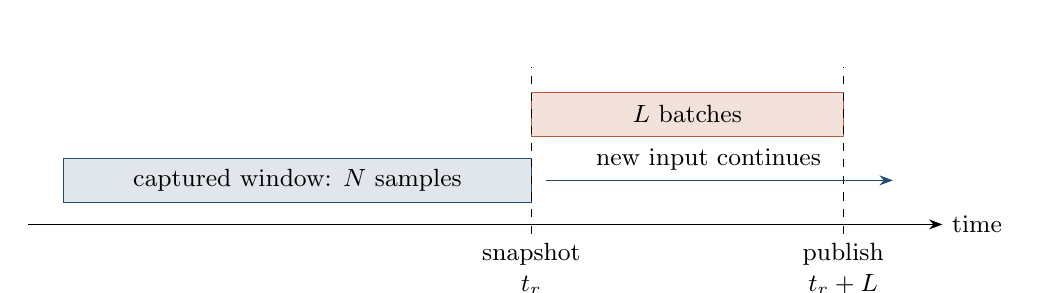
\begin{tikzpicture}[x=0.9cm,y=0.8cm,>=Stealth,font=\small]
\draw[->] (0,0)--(12.9,0) node[right] {time};
\fill[ink!14] (0.5,0.35) rectangle (7.1,1.05);
\draw[ink] (0.5,0.35) rectangle (7.1,1.05);
\node at (3.8,0.7) {captured window: $N$ samples};
\fill[accent!18] (7.1,1.4) rectangle (11.5,2.1);
\draw[accent] (7.1,1.4) rectangle (11.5,2.1);
\node at (9.3,1.75) {$L$ batches};
\draw[dashed] (7.1,-0.15)--(7.1,2.5);
\draw[dashed] (11.5,-0.15)--(11.5,2.5);
\node[below,align=center] at (7.1,-0.15) {snapshot\\$t_r$};
\node[below,align=center] at (11.5,-0.15) {publish\\$t_r+L$};
\draw[->,ink] (7.3,0.7)--(12.2,0.7);
\node[above] at (9.6,0.7) {new input continues};
\end{tikzpicture}
\caption{Logical timeline, not to scale. The transform operates on an owned copy of the captured frame while the input ring continues to advance. A smaller batch quota delays publication without changing that frame's spectral contents.}
\label{fig:timeline}
\end{figure}

\subsection{Consequences for temporal smoothing}
The modules use an exponential magnitude smoother. Writing its intended time
constant as $\tau$ and assuming a nominal interval $H/f_s$ gives
\begin{equation}
 y_r=\alpha y_{r-1}+(1-\alpha)|X_r|,\qquad
 \alpha=\exp[-H/(f_s\tau)].
\end{equation}
The implementation's user-facing smoothing-time parameter corresponds to
$10\tau$. If actual updates arrive every $L/f_s$, then after elapsed time $t$
the old state is attenuated approximately by
$\exp[-tH/(L\tau)]$. The effective time constant is thus
\begin{equation}
 \tau_{\mathrm{eff}}=\tau L/H.
\end{equation}
For the 4096-point example, the decay time is approximately 8.3\% shorter than
its nominal interpretation. An exact frame clock or elapsed-sample timestamps
would remove this discrepancy. The analysis also motivates timestamping
spectrogram columns by captured frames rather than assuming the configured
horizon is their spacing.

\subsection{Exact-horizon alternative}
If an application requires publication exactly every $H$ calls, it can separate
the frame clock from completion and retain a finished result until its scheduled
publication. Alternatively, for an ordered sequence of $B$ work units, assign
call $s\in\{1,\ldots,H\}$ the quota
\begin{equation}
 q_s=\floor{sB/H}-\floor{(s-1)B/H}.
 \label{eq:balanced}
\end{equation}
These quotas sum to $B$ by telescoping; each is either $\floor{B/H}$ or
$\ceil{B/H}$. For $B>0$, the last quota is positive, so the ordered work ends
on call $H$. Among schedules for $B$ unit-cost operations in $H$ calls, no
schedule can have a maximum quota smaller than $\ceil{B/H}$, by the pigeonhole
principle. Equation~\eqref{eq:balanced} attains that lower bound. This elementary
balanced schedule is a reference design, not a claimed new scheduling result
or a change to the shipped implementation. Its unit-cost premise does not make
unequal preparation and reconstruction operations interchangeable butterflies.

\section{Whole-Pipeline Cost and Ownership}
\label{sec:cost}
The real FFT's public interface exposes a useful but partial work budget.
A schematic call-cost model is
\begin{equation}
 C_s=C_{\mathrm{input},s}+C_{\mathrm{dispatch},s}
       +b_s C_{\mathrm{butterfly},s}
       +\mathbf{1}_{s=0}C_{\mathrm{prepare}}
       +\mathbf{1}_{s=L-1}C_{\mathrm{reconstruct}}
       +C_{\mathrm{publish},s}.
 \label{eq:cost}
\end{equation}
Here $b_s\le q$ is the number of useful butterflies, and costs need not be
constant across stages or calls. Publication of a previous result may coincide
with preparation of the next. The expression describes locations of work,
not a hardware-independent cycle prediction.

In the source snapshot, real-input packing creates a temporary vector;
copying and bit reversal are bulk operations; reconstruction is bulk; optional
fractional-octave smoothing allocates a prefix-sum array; temporal smoothing
and display-coordinate conversion visit complete arrays. Window-length
reconfiguration may resize storage on the engine path. The existing
implementation therefore does not satisfy an allocation-free, uniformly
small-call contract merely because its inner FFT is resumable.

If $H=\rho N$ for fixed $\rho>0$, then $q=\Theta(\log N)$ for the real FFT.
The butterfly work assigned to ordinary calls grows logarithmically, while
preparation and reconstruction still contribute $\Theta(N)$ operations to
boundary calls. Consequently, the full real-FFT path retains a linear peak
operation count under this scaling. The change from a full
$\Theta(N\log N)$ burst to smaller inner batches can still be useful, but the
asymptotic distinction must be stated at the correct boundary.

\subsection{Magnitude processing and SIMD}
Fractional-octave smoothing uses a prefix sum of magnitudes, allowing a range
mean to be evaluated with two prefix accesses after a linear setup pass. For
fraction $\beta$ of an octave, the nominal band around $f_k$ is
$[f_k2^{-\beta/2},f_k2^{\beta/2}]$, discretized to FFT-bin indices and adjusted
near Nyquist. The result is a visualization-oriented magnitude average, not a
constant-Q transform or a power-conserving spectral estimate. Phase is discarded
when smoothed magnitudes replace complex coefficients.

The Fourier module instantiates arithmetic on \code{simd::float\_4}. Each lane
carries an independent input channel through the same traversal; the SIMD
lanes are not four consecutive bins of one transform. This arrangement
shares index/control work across channels. It does not establish a measured
fourfold speedup, and the scalar experiments below do not validate Rack SIMD
instantiations. Rack's plugin API supplies the host processing and SIMD
context~\cite{rack}.

\subsection{Snapshots and publication}
The input ring can continue advancing because \code{buffer()} copies the
selected frame into transform-owned storage. Resuming directly from a mutable
ring without preserving the selected samples would violate
Equation~\eqref{eq:dft}. Any attempt to distribute packing must therefore solve
input lifetime as well as arithmetic scheduling.

Similarly, a display-readiness flag is not by itself an engine-to-display
synchronization protocol. Concurrent reads of arrays being modified require an
ownership and publication design consistent with the C++ memory model. The
current source's shared display buffers are not certified by the scalar tests.
A future implementation could publish completed immutable snapshots through a
bounded exchange of preallocated buffers, with an explicit policy for a slow
consumer. An atomic pointer alone would still require safe buffer reclamation.
No such handoff redesign is evaluated here.

\section{Experimental Method}
\label{sec:method}
The artifact contains a standalone C++11 driver and a Python standard-library
runner. The runner records source digests before compilation and rejects a run
if those files change during evaluation. No Rack headers, devices, or external
FFT libraries are required. The source is compiled using Apple Clang
21.0.0 (\code{clang-2100.1.1.101}), with
\code{-std=c++11 -O3 -DNDEBUG -Wall -Wextra -pedantic}; fast-math is not enabled.
The recorded host is an Apple M1 Pro with 16 GiB of memory, running macOS
26.6.2. Measurements were collected on September 28, 2026. No core affinity,
real-time thread policy, frequency locking, or exclusive machine reservation
was imposed.

\subsection{Numerical and schedule verification}
Lengths are all powers of two from 4 through 4096, using both \code{float}
and \code{double}. Fixtures are silence, an impulse, DC, a Nyquist alternating
sequence, a bin-centered sinusoidal mixture, and deterministic pseudorandom
samples. Each is tested with a rectangular window and a periodic Hann window.
The pseudorandom generator is the explicitly specified 32-bit recurrence in the
driver; it is not dependent on a standard library's distribution implementation.

For every fixture/window/precision/length combination, \code{compute()} is
compared bitwise against repeated \code{step(H)} for
$H\in\{1,N/4,N/2,N,N+7\}$. The list intentionally retains coincident horizons
at the smallest size. Every completion count is checked against
$\ceil{B_r/\ceil{B_r/H}}$. These checks examine the actual header, not a rewritten
FFT model.

For lengths through 128, a separately written $O(N^2)$ complex DFT checks every
output bin, including DC, Nyquist, and the conjugate half. The reference uses
the actual windowed input values presented to the FFT and reports
\begin{equation}
 E=\frac{\max_k|\widehat X[k]-X_{\mathrm{ref}}[k]|}
          {\max(1,\sum_m|u[m]|)}.
 \label{eq:error}
\end{equation}
The denominator avoids unstable relative error at spectral nulls. The acceptance
threshold is $64\epsilon_T$ for the tested scalar type; it is a regression
threshold for this small-size reference campaign, not a proven error bound for
all lengths. Although the reference uses \code{long double}, that type has 53
significand bits on this host. In particular, the double-precision reference is
an independent formulation, not a higher-precision oracle.

\subsection{Timing comparison}
The timing workload uses one scalar \code{float} real transform, lengths
$N\in\{1024,2048,4096,16384\}$, and horizons $H=N/4$ and $H=N/2$. A fixed
pseudorandom frame is multiplied by an explicitly constructed periodic Hann
window. Transform construction, table initialization, window construction, and
fixture generation are excluded. Packing allocation, window multiplication,
copying, bit reversal, and reconstruction are included.

Two modes share the same FFT implementation. The complete mode performs
\code{buffer()} followed by \code{compute()} in the first simulated sample
call. The incremental mode performs \code{buffer()} in that call and invokes
\code{step(H)} on all $H$ calls, retaining any early-completed result until the
next fixed frame boundary. This controlled cadence holds the number of frames
constant; it deliberately differs from the modules' immediate-restart behavior
so that a faster update rate does not confound the scheduling comparison.

Each mode receives 16 warmup transforms and two measured passes of 64 frames.
The first pass times whole frames with no clock reads inside the incremental
loop; the complete baseline has no FFT work in the other $H-1$ logical calls.
The second pass times every simulated call, records preparation and completing
calls separately, and retains per-run p99 and maximum durations. Output
magnitudes are consumed through a volatile checksum outside the timed regions
to prevent dead-code elimination. Both modes compute full spectra.

There are nine paired repetitions per size/horizon combination. Execution order
alternates between complete-first and incremental-first on successive
repetitions. Results include medians and full ranges across repetitions. For
paired ratios, the runner resamples the nine pairs 10,000 times with a fixed
seed and reports percentile bootstrap intervals. These intervals describe
within-session repeat variability; they do not account for different hardware,
operating systems, compilers, or background loads.

The timer is \code{std::chrono::steady\_clock}. An empty start/end pair has median
0 ns and p99 42 ns in the recorded calibration. Tiny per-call observations are
therefore quantized and instrumentation-sensitive. Clock overhead is not
subtracted. The separate frame pass avoids multiplying those clock reads by
$H$ when estimating aggregate work.

\section{Results}
\subsection{Numerical agreement and completion}
All 1320 incremental-versus-complete schedule cases passed, with bitwise-identical
completed spectra within each tested type. The independent reference checked
6048 complex bins across both precisions. The maximum scaled errors were
$8.69\times10^{-8}$ for float (rounded upward) and
$1.06\times10^{-14}$ for double (rounded upward). These measurements support
correctness for the tested fixtures, sizes, and windows; they do not replace an
error analysis of every supported type or the module's amplitude calibration.

The schedule tests confirm Table~\ref{tab:cadence} and the distinction between
``no later than $H$'' and ``exactly at $H$.'' Increasing the requested horizon
can leave the actual completion interval unchanged until the integer quota
changes. Thus frame rate is a staircase function of the horizon under
completion-driven restarts, not generally its reciprocal.

\subsection{Peak work placement}
Table~\ref{tab:timing} reports the $H=N/2$ subset; the artifact also contains
$H=N/4$. Figure~\ref{fig:peaks} includes the full range of observed maxima across
repetitions. The median of run maxima is much smaller in incremental mode,
but individual maxima vary considerably. At $N=2048$, for example, one
incremental run reaches 21.209 microseconds even though its median run maximum
is 1.625 microseconds. Such observations are consistent with an ordinary
scheduled process and are retained rather than removed as outliers.

\begin{table}[tb]
\centering\small
\begin{tabular}{@{}rrr rrr@{}}
\toprule
& \multicolumn{2}{c}{Frame time ($\mu$s)} & \multicolumn{2}{c}{Run maximum ($\mu$s)} & Peak ratio \\
\cmidrule(lr){2-3}\cmidrule(lr){4-5}
$N$ & Complete & Incremental & Complete & Incremental & Paired 95\% interval \\
\midrule
1,024 & 7.619 & 7.518 & 7.917 & 0.875 & [0.083, 0.508] \\
2,048 & 16.662 & 15.915 & 17.291 & 1.625 & [0.091, 0.111] \\
4,096 & 36.620 & 35.603 & 39.458 & 3.333 & [0.079, 0.296] \\
16,384 & 169.510 & 163.844 & 179.625 & 13.125 & [0.073, 0.113] \\
\bottomrule
\end{tabular}
\caption{Medians across nine repetitions, $H=N/2$. Frame time comes from the aggregate pass; run maximum comes from the separately instrumented pass. Intervals are bootstrap intervals for the median paired incremental/complete run-maximum ratio, not ratios of the displayed marginal medians and not worst-case bounds.}
\label{tab:timing}
\end{table}

\begin{figure}[tb]
\centering
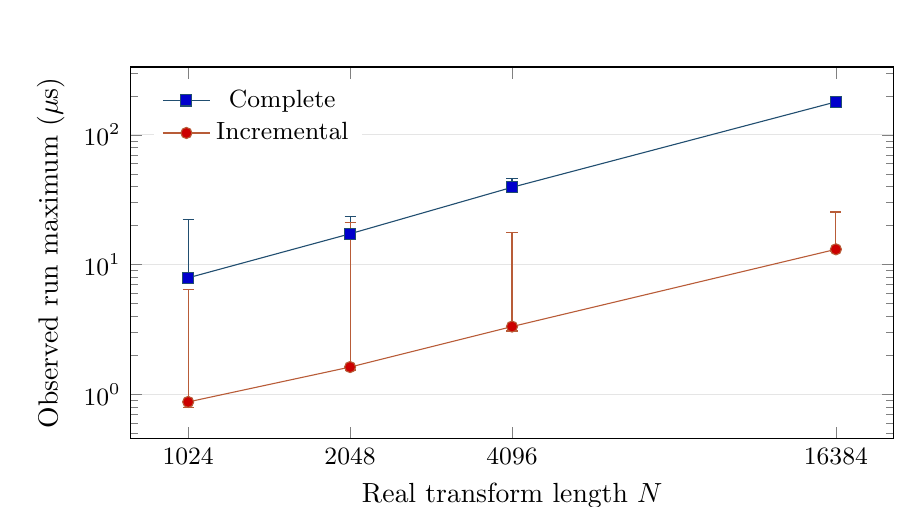
\begin{tikzpicture}
\begin{axis}[width=0.93\linewidth,height=6.3cm,ymode=log,xmode=log,log basis x=2,
 ylabel={Observed run maximum ($\mu$s)},xlabel={Real transform length $N$},
 xtick={1024,2048,4096,16384},xticklabels={1024,2048,4096,16384},xmin=800,xmax=21000,
 ymajorgrids=true,grid style={black!10},legend pos=north west,
 legend style={draw=none,font=\small},tick label style={font=\small}]
\addplot+[color=ink,mark=square*,error bars/.cd,y dir=both,y explicit]
 coordinates {(1024,7.917) += (0,14.374) -= (0,0.167)
 (2048,17.291) += (0,6.084) -= (0,0.457)
 (4096,39.458) += (0,6.751) -= (0,1.958)
 (16384,179.625) += (0,13.084) -= (0,7.959)};
\addlegendentry{Complete}
\addplot+[color=accent,mark=*,error bars/.cd,y dir=both,y explicit]
 coordinates {(1024,0.875) += (0,5.584) -= (0,0.083)
 (2048,1.625) += (0,19.584) -= (0,0.083)
 (4096,3.333) += (0,14.333) -= (0,0.249)
 (16384,13.125) += (0,12.333) -= (0,0.542)};
\addlegendentry{Incremental}
\end{axis}
\end{tikzpicture}
\caption{Median and full min--max range of per-run maximum call duration over nine repetitions, $H=N/2$. Vertical bars are observed ranges, not confidence intervals. Both axes are logarithmic; horizontal ticks identify the actual transform lengths. Measurements include RFFT preparation and reconstruction, but exclude module smoothing and graphics preparation.}
\label{fig:peaks}
\end{figure}

The incremental preparation-call medians are 0.542, 1.125, 2.709, and
10.667 microseconds for the four lengths. Completing-call medians are 0.750,
1.500, 3.042, and 12.375 microseconds. Their growth is consistent with the bulk
work identified by source analysis, although timings alone do not prove an
asymptotic bound. Distributing only the butterfly traversal leaves both ends of
the transform visible in the cost profile.

A striking measurement pitfall is that the median per-run p99 is approximately
42 ns for \emph{both} modes at all four lengths in this subset. The complete
mode's expensive call occurs only once per $H$ calls, below the top one percent
for these horizons. A p99-only comparison would largely miss the burst being
studied. Phase-specific measurements and run maxima are needed alongside
quantiles; none of them by itself is a proven worst-case execution time.

\subsection{Aggregate work and interpretation}
The median paired incremental/complete frame-time ratios for increasing $N$
are approximately 0.979, 0.955, 0.972, and 0.967. The corresponding percentile
intervals are [0.973, 1.005], [0.955, 0.956], [0.960, 0.977], and
[0.963, 0.968]. These modest differences are specific to the two loop structures
as optimized by this compiler on this workload. They do not indicate a reduction
in the butterfly count, nor establish an algorithmic throughput advantage. A
different compiler, batching policy, cache state, or vectorized library could
reverse the result. The robust interpretation of this campaign is the change
in work placement within this implementation, with broadly comparable total
frame cost.

The experiments use repeated fixed inputs, warm tables, and a scalar standalone
process. They omit ring insertion, Rack parameter access, SIMD channels,
frequency/time smoothing, display conversion, GUI consumption, and other
modules. They therefore cannot establish whole-patch dropout rates or a maximum
number of safe analyzer instances. No numerical value in this report is a
measurement from a running Rack session.

\section{Engineering Implications and Limits}
A resumable FFT is most attractive when a caller can tolerate delayed analysis,
wants explicit control of work on its existing thread, and needs complete
spectra at a modest frame rate. Whether it is preferable to an optimized batch
FFT depends on the actual callback budget and host scheduling model. If a
batch transform already fits comfortably, the extra state and cadence policy
may provide little practical benefit. For a small set of frequently updated
bins, a sliding formulation can be a more appropriate starting point. For
large analysis tasks, a worker may offer a better throughput/latency tradeoff
when the host permits it.

Sample-call costs should also not be confused with device-buffer deadlines.
If the host renders $K$ samples in one device callback, its relevant demand is
the sum of the associated module work over those $K$ samples, plus other engine
costs. A device callback containing preparation and reconstruction can still
experience a substantial burst. A future host study should vary $K$, frame
phase, analyzer count, and background patch load rather than extrapolating
from one scalar-call maximum.

A stronger implementation would make the analysis pipeline an explicit sequence
of owned stages: capture/packing, permutation, butterflies, reconstruction,
magnitude processing, and publication. Each stage would have a bounded chunk
size, preallocated storage, and well-defined completion and cancellation
semantics. Work units with very different costs would need separate budgets or
calibrated weights. Even then, empirical cost calibration would not guarantee
worst-case execution on a general-purpose operating system.

Exact cadence should be specified independently of scheduling: a frame-start
counter can define analysis timestamps, while the work scheduler merely ensures
completion before publication. If processing falls behind, the implementation
must choose whether to skip a frame, retain an older spectrum, or signal an
overrun; silently overwriting an unfinished frame changes the result. Reset,
sample-rate changes, and FFT-length changes likewise require explicit
cancellation/reinitialization behavior. These are proposed design requirements,
not features demonstrated by this artifact.

The principal limitations of the evidence are its single host and compiler,
small number of repeated runs, same-session resampling, absence of an optimized
library baseline, and absence of an end-to-end Rack workload. The numerical
campaign uses independent direct transforms only for small sizes; large-size
checks establish schedule equivalence rather than independent correctness.
The report also does not evaluate non-power-of-two lengths, forward-path invalid
inputs, multithreaded access, inverse reconstruction applications, or
calibration accuracy of every window/display setting.

\section{Conclusion}
Fourier illustrates how a conventional FFT can become a schedulable component
by exposing its traversal state. The resulting operation-count budget has a
simple completion proof and preserves the order of arithmetic. Its application
also exposes two easily overlooked distinctions: completing within a requested
horizon is not the same as maintaining that frame interval, and budgeting
butterflies is not the same as budgeting a complete analysis pipeline.

The recorded experiments support the practical value of redistributing work
within this scalar implementation, while the source analysis explains the
remaining linear-time boundary costs. The useful contribution is a transparent
account of these tradeoffs, backed by executable evidence and explicit limits.
A fully bounded implementation would extend the same scheduling discipline to
preparation, reconstruction, publication, and the lifetime of every shared
buffer.

\appendix
\section{Reproducibility and Source Map}
The code artifact is available at \repo. All report sources and experiment data
are in \code{whitepaper/}. The manuscript embeds its figures, listings, and
bibliography so that one \code{.tex} file suffices for typesetting; compilation
does not run experiments or fetch network resources.

From the repository root, reproduce the numerical and timing campaign with:
\begin{lstlisting}[language=bash]
python3 whitepaper/experiments/run.py --cpu "YOUR CPU MODEL" \
    --memory-gib 16
\end{lstlisting}
Replace the illustrative hardware fields with the actual host values. New
results go to \path{whitepaper/build/evaluation/}; the archived
\path{whitepaper/data/} files remain unchanged. The runner honors \code{CXX}
and records the actual compiler and command. The original command used
\code{--cpu "Apple M1 Pro" --memory-gib 16}. Both passes must be interpreted
using the methodology in Section~\ref{sec:method}, including the intentionally
fixed cadence.

The primary implementation paths are \path{src/dsp/math/fft.hpp},
\path{src/SpectrumAnalyzer.cpp}, and \path{src/Spectrogram.cpp}.
\path{src/dsp/math/window.hpp} provides cached windows;
\path{src/dsp/math/circular_buffer.hpp} provides the contiguous ring.
The independent report driver is \path{whitepaper/experiments/evaluate.cpp}.
\code{metadata.json} records the revision, header/driver hashes, compiler,
hardware declaration, timestamps, and raw-data hashes. \code{timing.csv} stores
all 144 mode/repetition observations; \code{verification.csv} stores all 22
precision/length summaries. \code{summary.json} stores derived statistics and
bootstrap intervals. The archived data are observations, not portable timing
requirements.

\section{Data and Software Availability}
The source code is distributed under GPL-3.0-or-later; the repository's license
file documents separate visual-asset terms. The diagrams in this report are
original vector illustrations and do not reproduce plugin artwork. The report
is a technical manuscript, not a claim of journal acceptance or arXiv deposit.
Use this report as the single citation for the work. Reference the supporting
code artifact through the GitHub link above and identify the software version
or commit used for reproducibility; no separate software citation is needed.
The repository's citation metadata provides the same report citation.
A persistent public report identifier can be added after deposit without
changing the title or author identity.

\begin{thebibliography}{99}
\small\raggedright
\bibitem{cooley1965}
J. W. Cooley and J. W. Tukey, ``An algorithm for the machine calculation of
complex Fourier series,'' \emph{Mathematics of Computation}, vol. 19, no. 90,
pp. 297--301, 1965. \href{https://doi.org/10.1090/S0025-5718-1965-0178586-1}{doi:10.1090/S0025-5718-1965-0178586-1}.

\bibitem{sorensen1987}
H. V. Sorensen, D. L. Jones, M. T. Heideman, and C. S. Burrus,
``Real-valued fast Fourier transform algorithms,'' \emph{IEEE Transactions
on Acoustics, Speech, and Signal Processing}, vol. 35, no. 6, pp. 849--863,
1987. \href{https://doi.org/10.1109/TASSP.1987.1165220}{doi:10.1109/TASSP.1987.1165220}.

\bibitem{allen1977}
J. B. Allen and L. R. Rabiner, ``A unified approach to short-time Fourier
analysis and synthesis,'' \emph{Proceedings of the IEEE}, vol. 65, no. 11,
pp. 1558--1564, 1977.
\href{https://doi.org/10.1109/PROC.1977.10770}{doi:10.1109/PROC.1977.10770}.

\bibitem{harris1978}
F. J. Harris, ``On the use of windows for harmonic analysis with the discrete
Fourier transform,'' \emph{Proceedings of the IEEE}, vol. 66, no. 1,
pp. 51--83, 1978.
\href{https://doi.org/10.1109/PROC.1978.10837}{doi:10.1109/PROC.1978.10837}.

\bibitem{lo1998}
P.-C. Lo and Y.-Y. Lee, ``Real-time implementation of the split-radix FFT---an
algorithm to efficiently construct local butterfly modules,''
\emph{Signal Processing}, vol. 71, no. 3, pp. 291--299, 1998.
\href{https://doi.org/10.1016/S0165-1684(98)00152-2}{doi:10.1016/S0165-1684(98)00152-2}.

\bibitem{lo1999}
P.-C. Lo and Y.-Y. Lee, ``Real-time FFT algorithm applied to on-line spectral
analysis,'' \emph{Circuits, Systems, and Signal Processing}, vol. 18, no. 4,
pp. 377--393, 1999.
\href{https://doi.org/10.1007/BF01200789}{doi:10.1007/BF01200789}.

\bibitem{lomoving1999}
P.-C. Lo and Y.-Y. Lee, ``Real-time implementation of the moving FFT
algorithm,'' \emph{Signal Processing}, vol. 79, no. 3, pp. 251--259, 1999.
\href{https://doi.org/10.1016/S0165-1684(99)00098-5}{doi:10.1016/S0165-1684(99)00098-5}.

\bibitem{hurchalla2010}
J. Hurchalla, ``A time distributed FFT for efficient low latency convolution,''
in \emph{129th Audio Engineering Society Convention}, paper 8257, 2010.
\url{https://secure.aes.org/forum/pubs/conventions/?elib=15679}.

\bibitem{battenberg2011}
E. Battenberg and R. Avi\v{z}ienis, ``Implementing real-time partitioned
convolution algorithms on conventional operating systems,'' in
\emph{Proceedings of the 14th International Conference on Digital Audio
Effects (DAFx-11)}, Paris, France, September 2011.
\url{https://ericbattenberg.com/pdf/partconvDAFx2011.pdf}.

\bibitem{liu2017}
J. Liu, B. Yan, and Q. Zou, ``Optimal time-distributed fast Fourier transform:
Application to online iterative learning control---experimental high-speed
nanopositioning example,'' \emph{Mechatronics}, vol. 41, pp. 114--124, 2017.
\href{https://doi.org/10.1016/j.mechatronics.2016.11.007}{doi:10.1016/j.mechatronics.2016.11.007}.

\bibitem{jacobsen2003}
E. Jacobsen and R. Lyons, ``The sliding DFT,'' \emph{IEEE Signal Processing
Magazine}, vol. 20, no. 2, pp. 74--80, 2003.
\href{https://doi.org/10.1109/MSP.2003.1184347}{doi:10.1109/MSP.2003.1184347}.

\bibitem{jacobsen2015}
E. Jacobsen, ``Understanding and implementing the sliding DFT,''
\emph{DSPRelated}, 2015.
\url{https://www.dsprelated.com/showarticle/776.php}.

\bibitem{richardson2019}
L. F. Richardson and W. F. Eddy, ``Algorithm 991: The 2D tree sliding window
discrete Fourier transform,'' \emph{ACM Transactions on Mathematical Software},
vol. 45, no. 1, article 12, 2019.
\href{https://doi.org/10.1145/3264426}{doi:10.1145/3264426}.
Preprint: \url{https://arxiv.org/abs/1707.08213}.

\bibitem{frigo2005}
M. Frigo and S. G. Johnson, ``The design and implementation of FFTW3,''
\emph{Proceedings of the IEEE}, vol. 93, no. 2, pp. 216--231, 2005.
\href{https://doi.org/10.1109/JPROC.2004.840301}{doi:10.1109/JPROC.2004.840301}.

\bibitem{rack}
VCV, ``Plugin API guide,'' \emph{VCV Rack Manual}. Accessed September 28, 2026.
\url{https://vcvrack.com/manual/PluginGuide}.
\end{thebibliography}
\end{document}
